\section*{Problema 01}

\textbf{Explora en
	\url{https://colab.research.google.com/drive/1pwCqLdvxeqChzDG3MoFIgR7m6lsInKs5?usp=sharing} el efecto de cambiar los parámetros en una SVM y convéncete que es de acuerdo a (congruente con) el funcional de costo de una SVM.}

\subsection*{Experimento 1}

\textbf{¿Cuál es el efecto de cambiar el parámetro $\lambda$/$\gamma$ (cost)?}

\begin{figure}[H]
	\centering
	\begin{subfigure}{0.24\linewidth}
		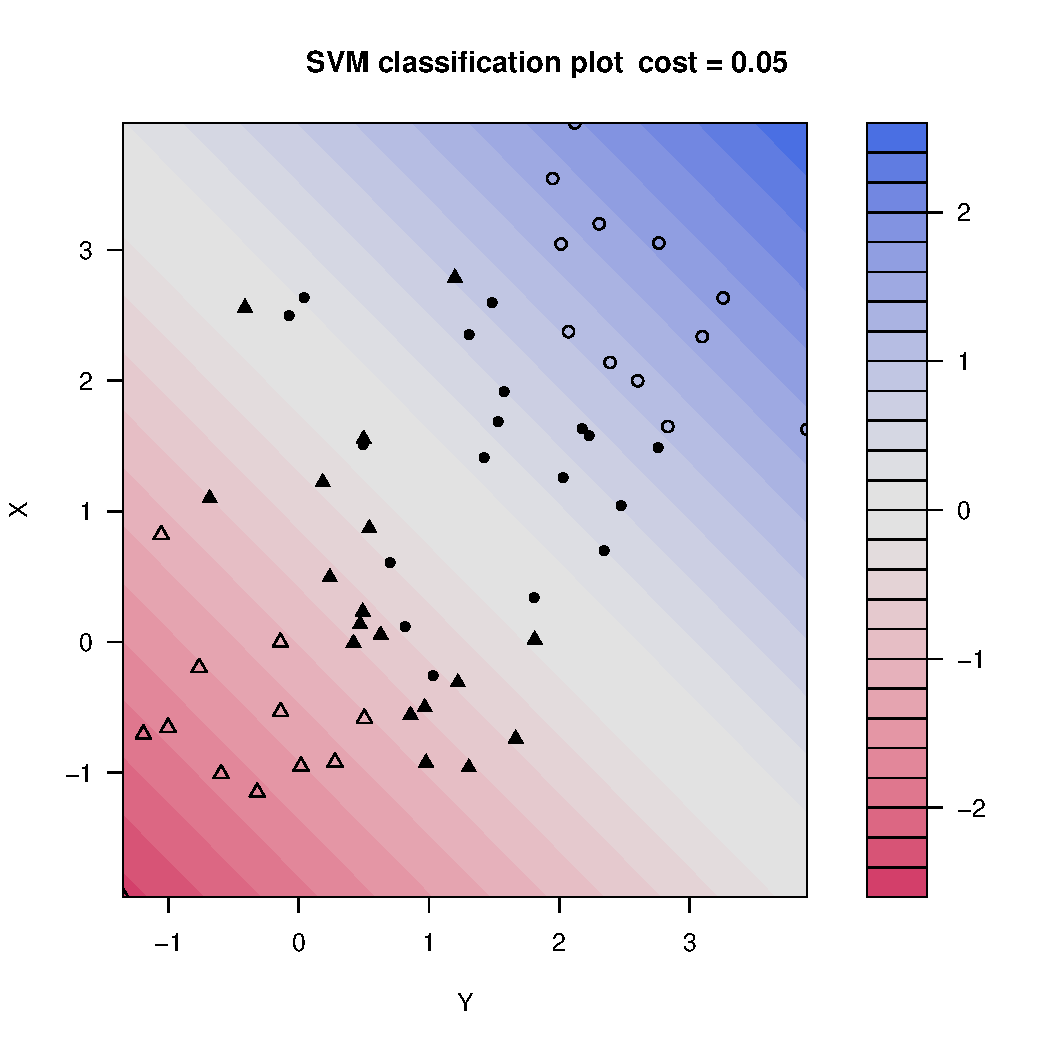
\includegraphics[width=1\linewidth]{Graphics/Problema_01/Experiment_01_1.pdf}
		\caption{Costo igual a 0.05}
	\end{subfigure}
	\begin{subfigure}{0.24\linewidth}
		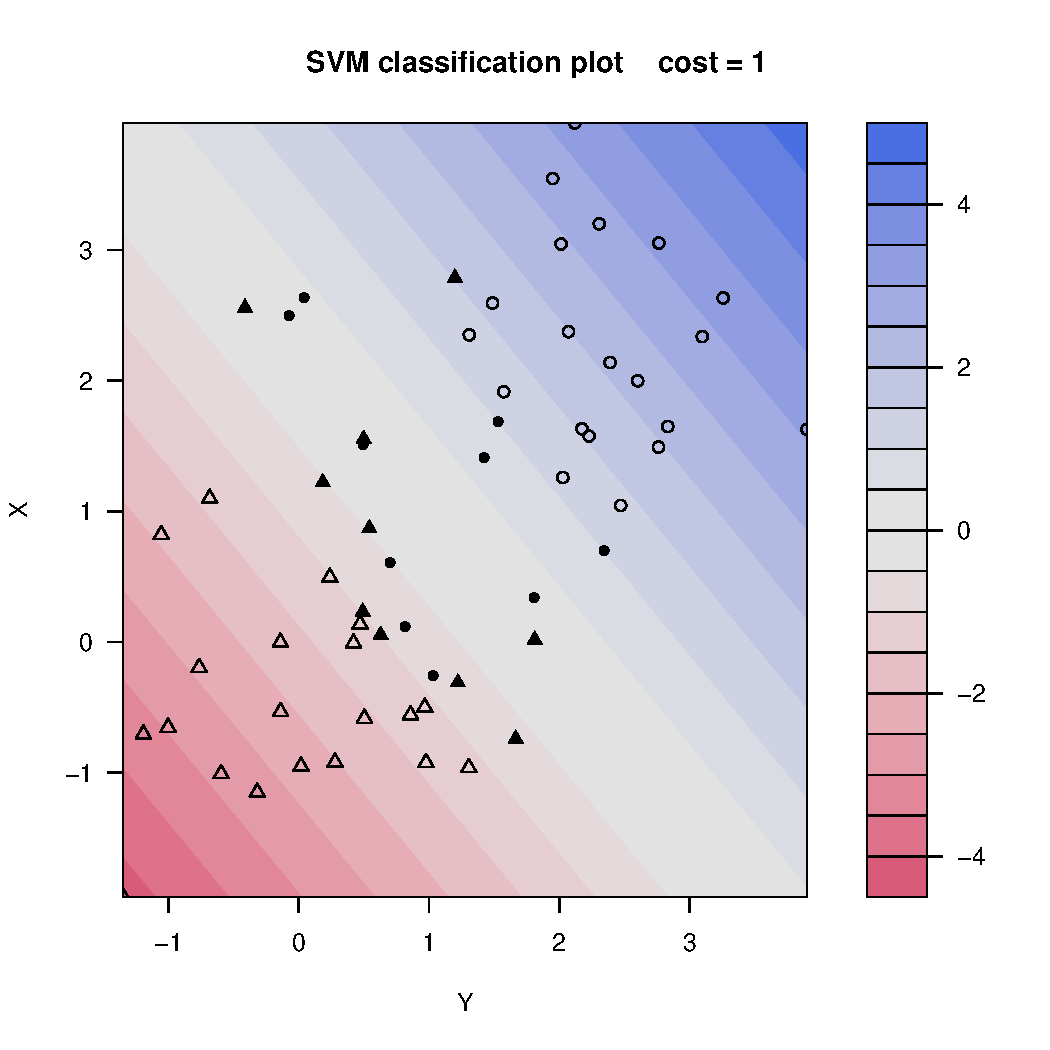
\includegraphics[width=1\linewidth]{Graphics/Problema_01/Experiment_01_2.pdf}
		\caption{Costo igual a 1}
	\end{subfigure}
	\begin{subfigure}{0.24\linewidth}
		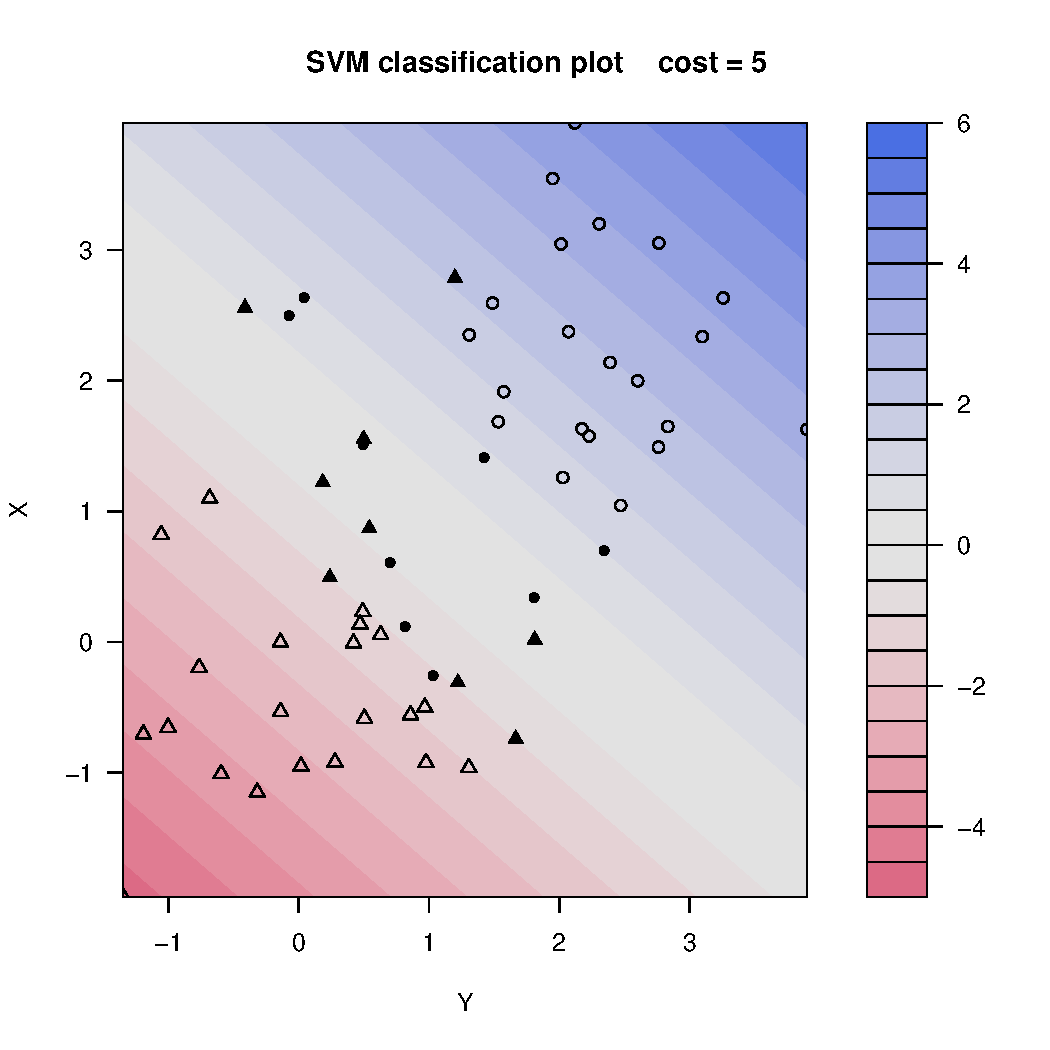
\includegraphics[width=1\linewidth]{Graphics/Problema_01/Experiment_01_3.pdf}
		\caption{Costo igual a 5}
	\end{subfigure}
	\begin{subfigure}{0.24\linewidth}
		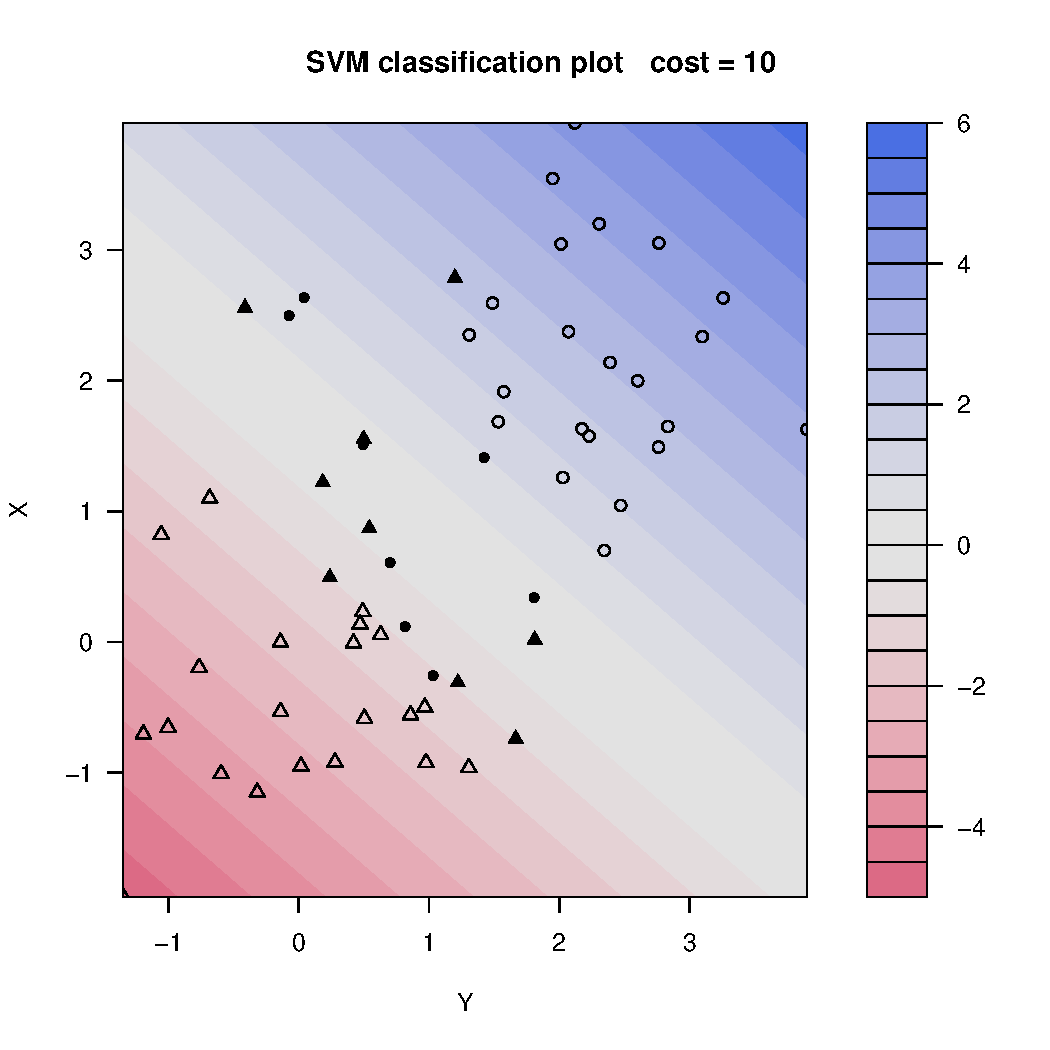
\includegraphics[width=1\linewidth]{Graphics/Problema_01/Experiment_01_4.pdf}
		\caption{Costo igual a 10}
	\end{subfigure}
	\caption{Diferentes valores de $\lambda / \gamma$ para el kernel lineal.}
	\label{fig:experimento_1}
\end{figure}

En la figura \ref{fig:experimento_1} se observa que conforme se aumenta el parámetro $\lambda / \gamma$ el número de vectores de soporte disminuye.

\subsection*{Experimento 2}

\textbf{¿Cuál es el efecto de aumentar el grado de polinomio?}

\begin{figure}[H]
	\centering
	\begin{subfigure}{0.24\linewidth}
		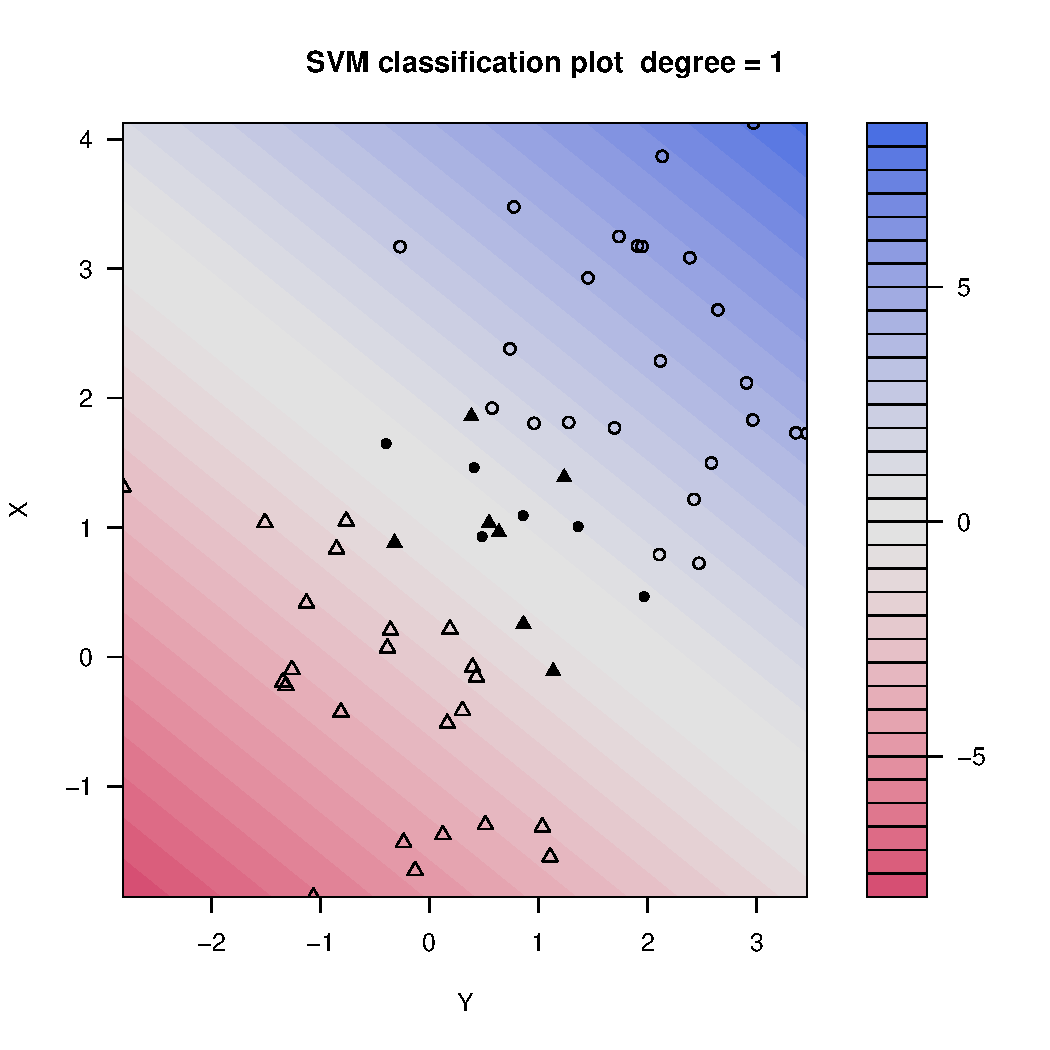
\includegraphics[width=1\linewidth]{Graphics/Problema_01/Experiment_02_1.pdf}
		\caption{Polinomio grado 1}
	\end{subfigure}
	\begin{subfigure}{0.24\linewidth}
		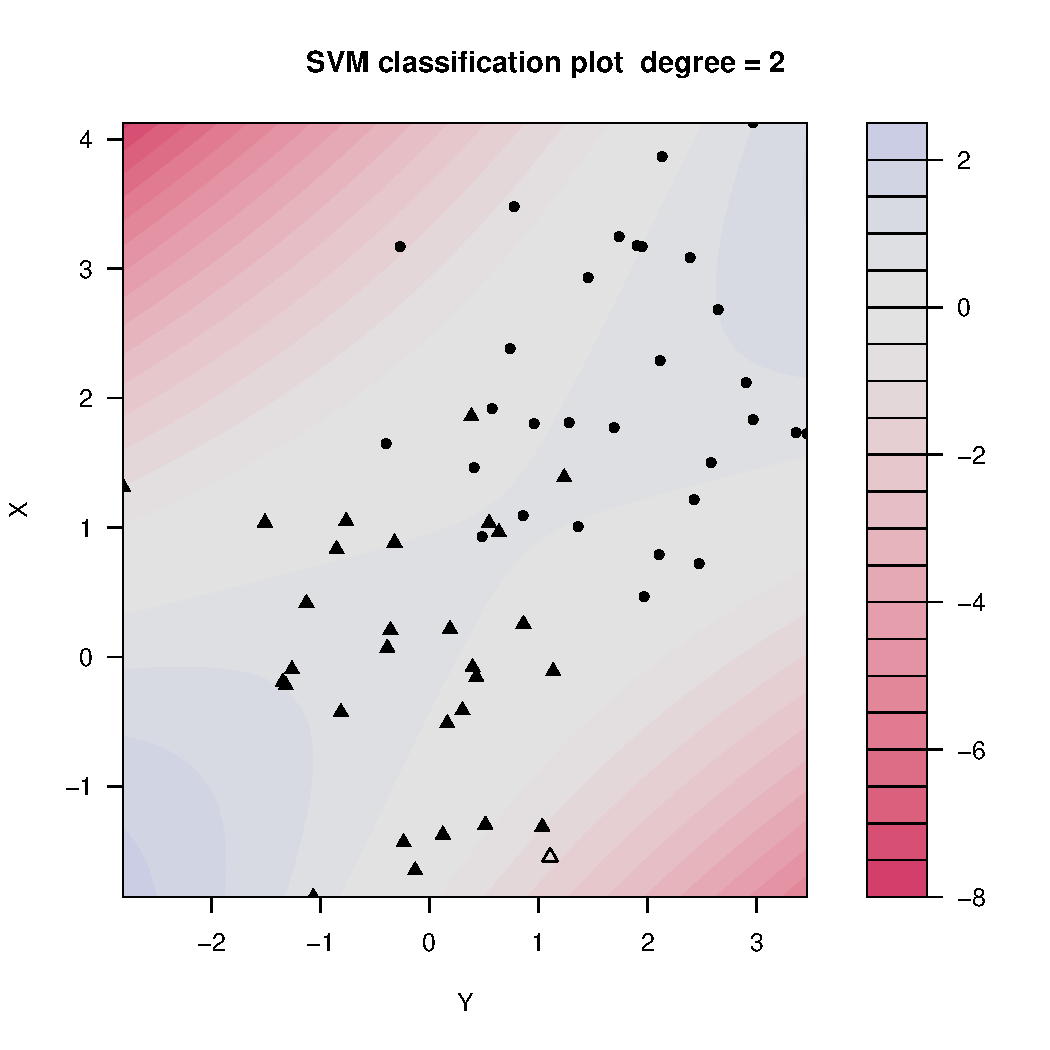
\includegraphics[width=1\linewidth]{Graphics/Problema_01/Experiment_02_2.pdf}
		\caption{Polinomio grado 2}
	\end{subfigure}
	\begin{subfigure}{0.24\linewidth}
		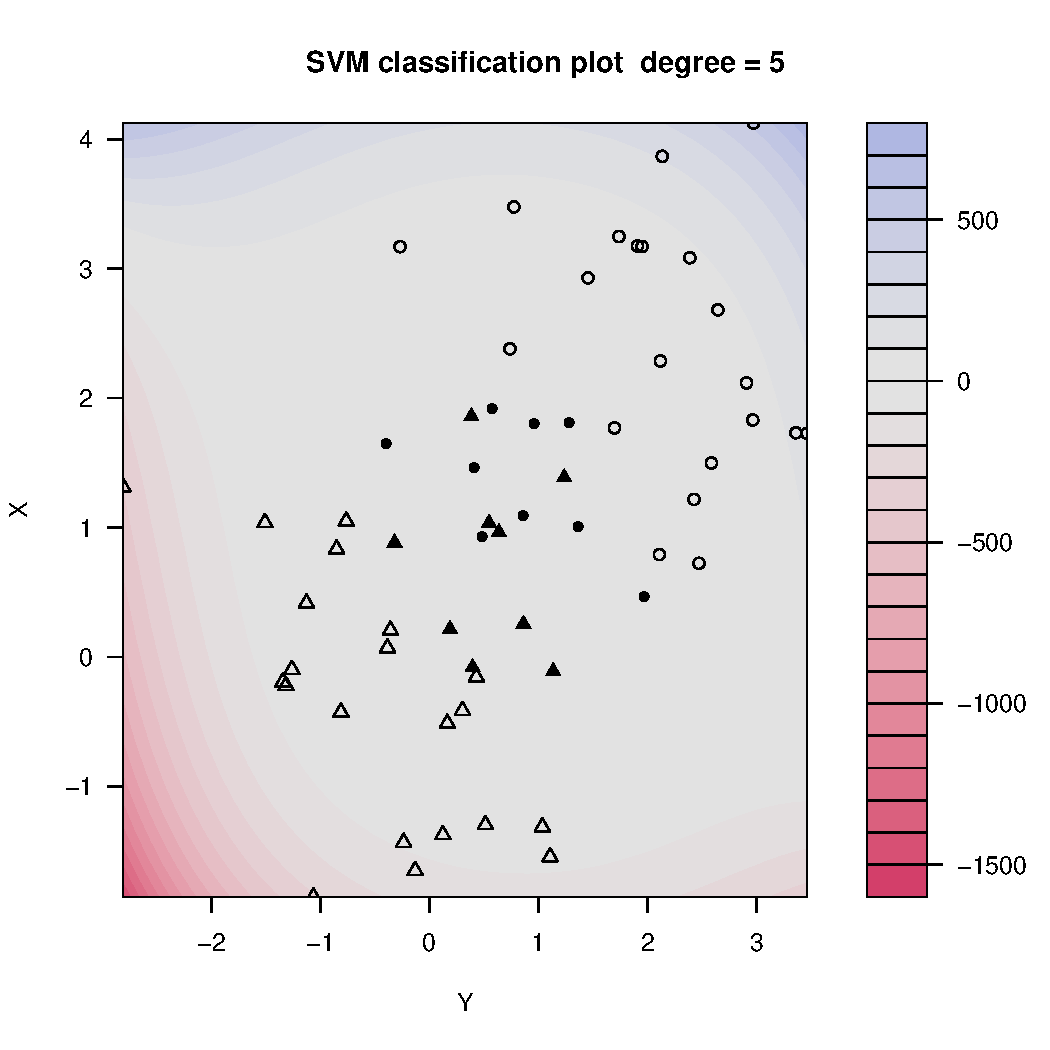
\includegraphics[width=1\linewidth]{Graphics/Problema_01/Experiment_02_3.pdf}
		\caption{Polinomio grado 5}
	\end{subfigure}
	\begin{subfigure}{0.24\linewidth}
		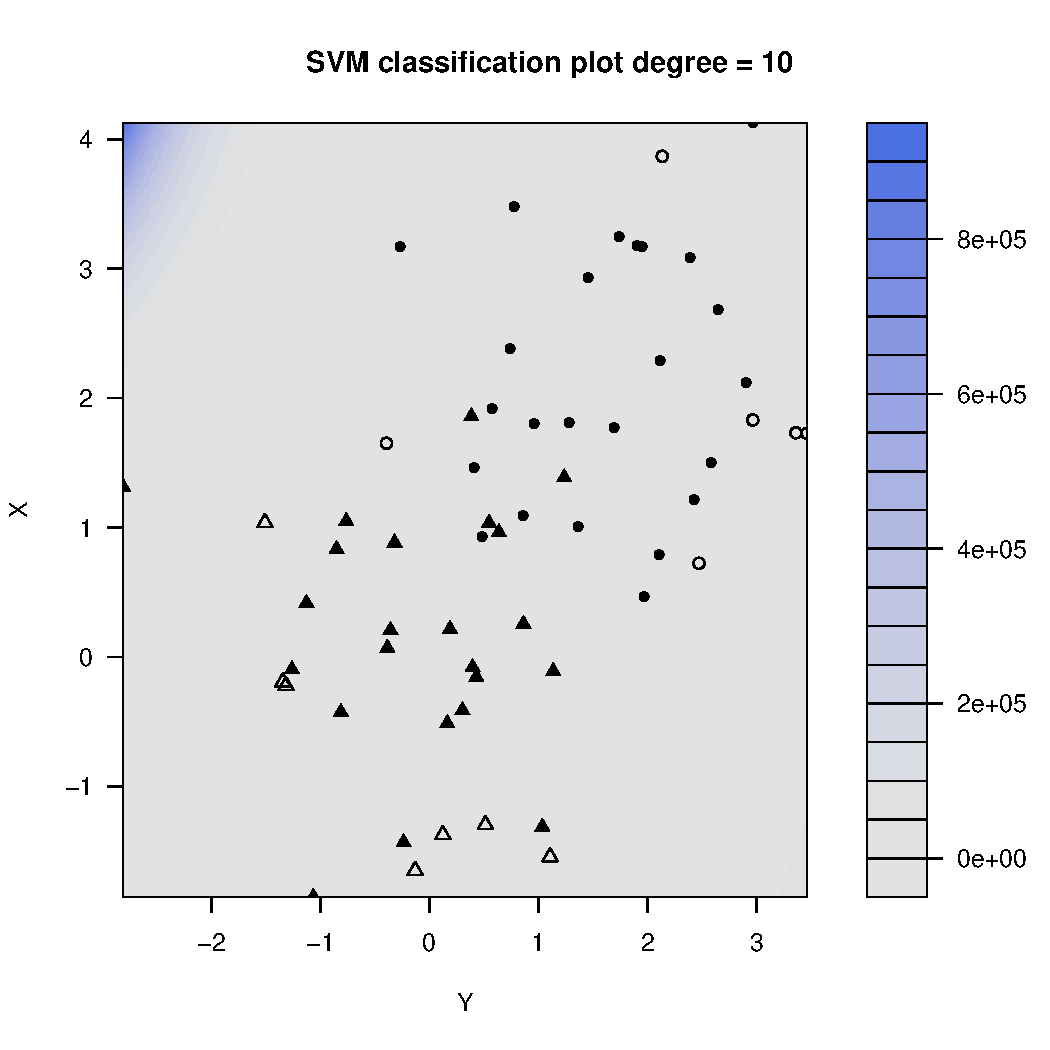
\includegraphics[width=1\linewidth]{Graphics/Problema_01/Experiment_02_4.pdf}
		\caption{Polinomio grado 10}
	\end{subfigure}
	\caption{Diferentes grados para el kernel polinomial.}
	\label{fig:experimento_2}
\end{figure}

En la figura \ref{fig:experimento_2} se observa que conforme se aumenta el grado del kernel polinomial, la región de clasificación para cada conjunto de datos se disuelve llegando a que todos los datos conforman un mismo conjunto.

\subsection*{Experimento 3}

\textbf{¿Cuál es el efecto de cambiar el parámetro $\sigma$ de kernel de base radial?}

\begin{figure}[H]
	\centering
	\begin{subfigure}{0.24\linewidth}
		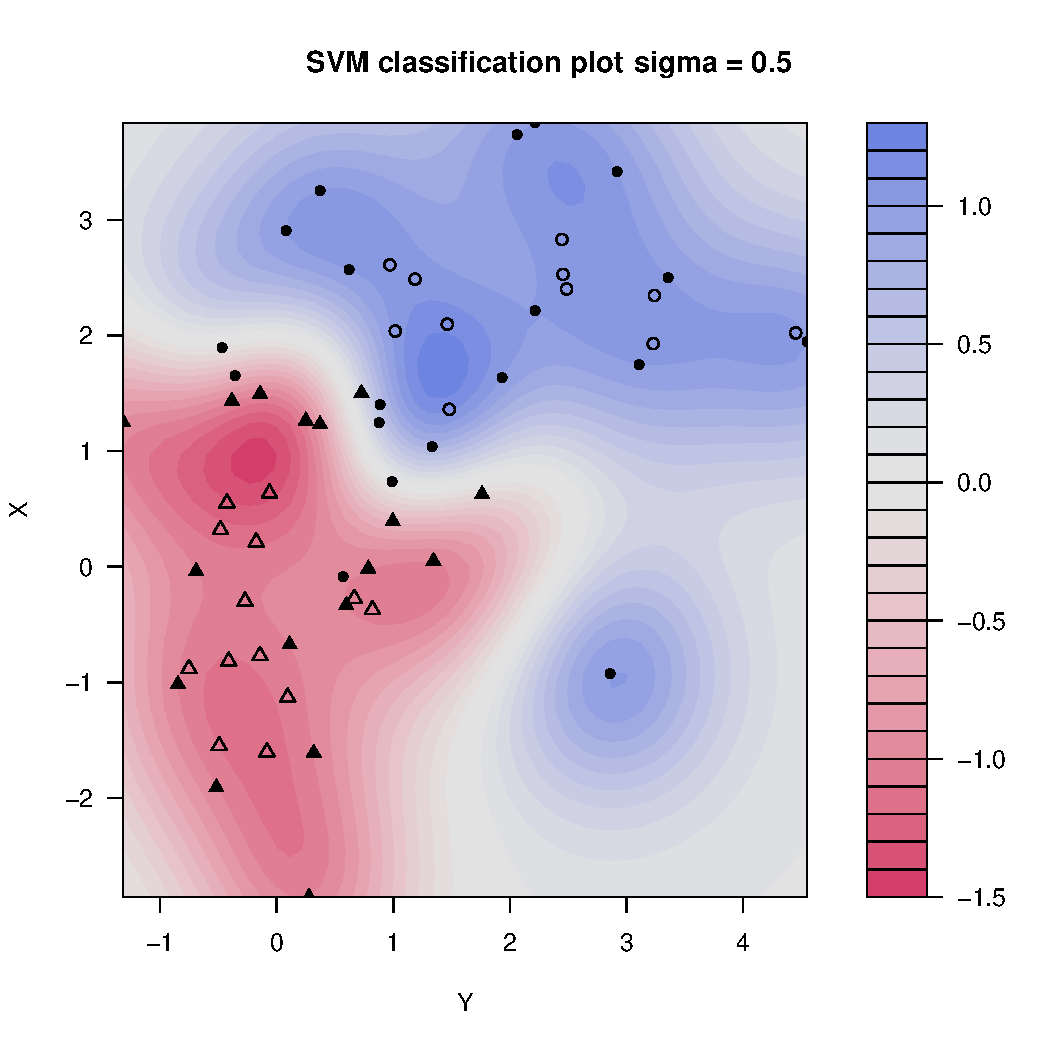
\includegraphics[width=1\linewidth]{Graphics/Problema_01/Experiment_03_1.pdf}
		\caption{$\sigma=0.5$}
	\end{subfigure}
	\begin{subfigure}{0.24\linewidth}
		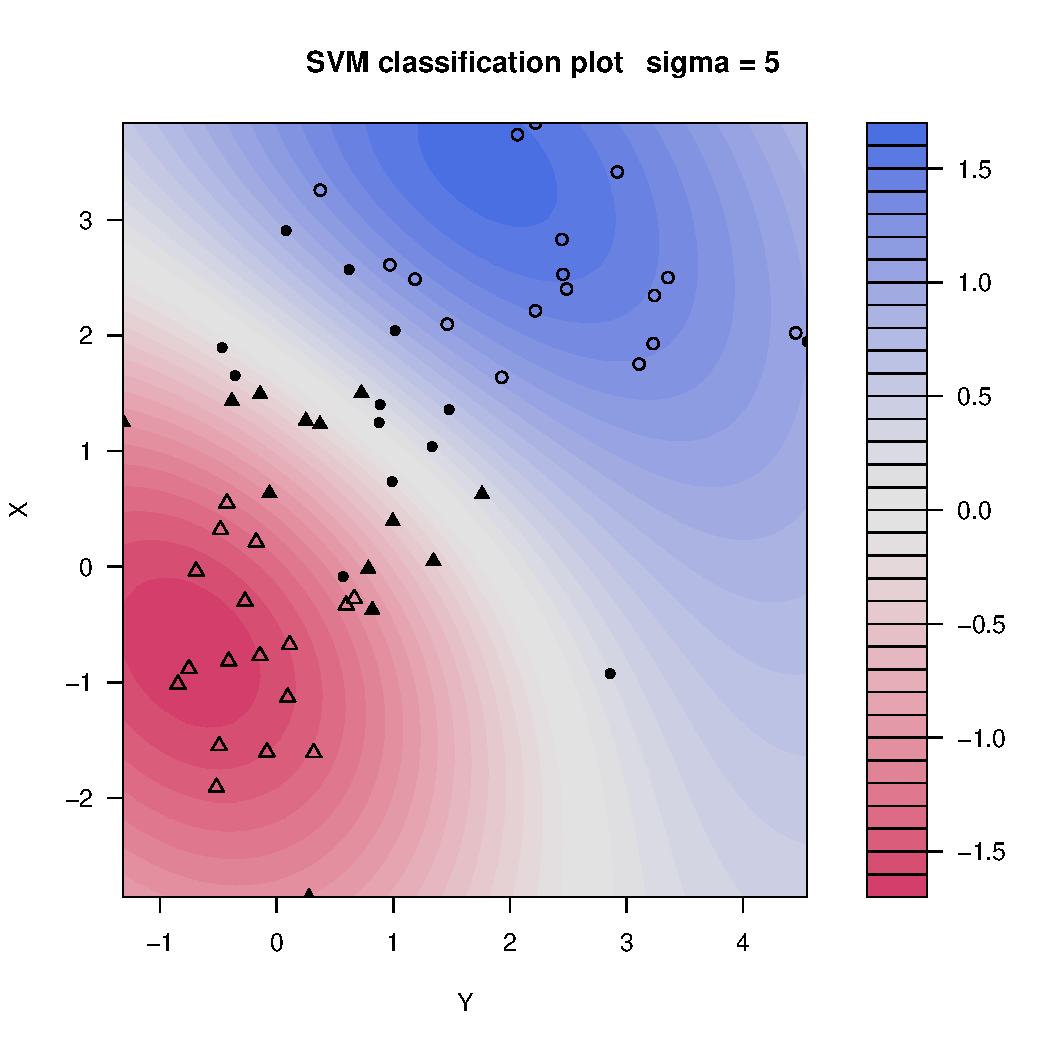
\includegraphics[width=1\linewidth]{Graphics/Problema_01/Experiment_03_2.pdf}
		\caption{$\sigma=5$}
	\end{subfigure}
	\begin{subfigure}{0.24\linewidth}
		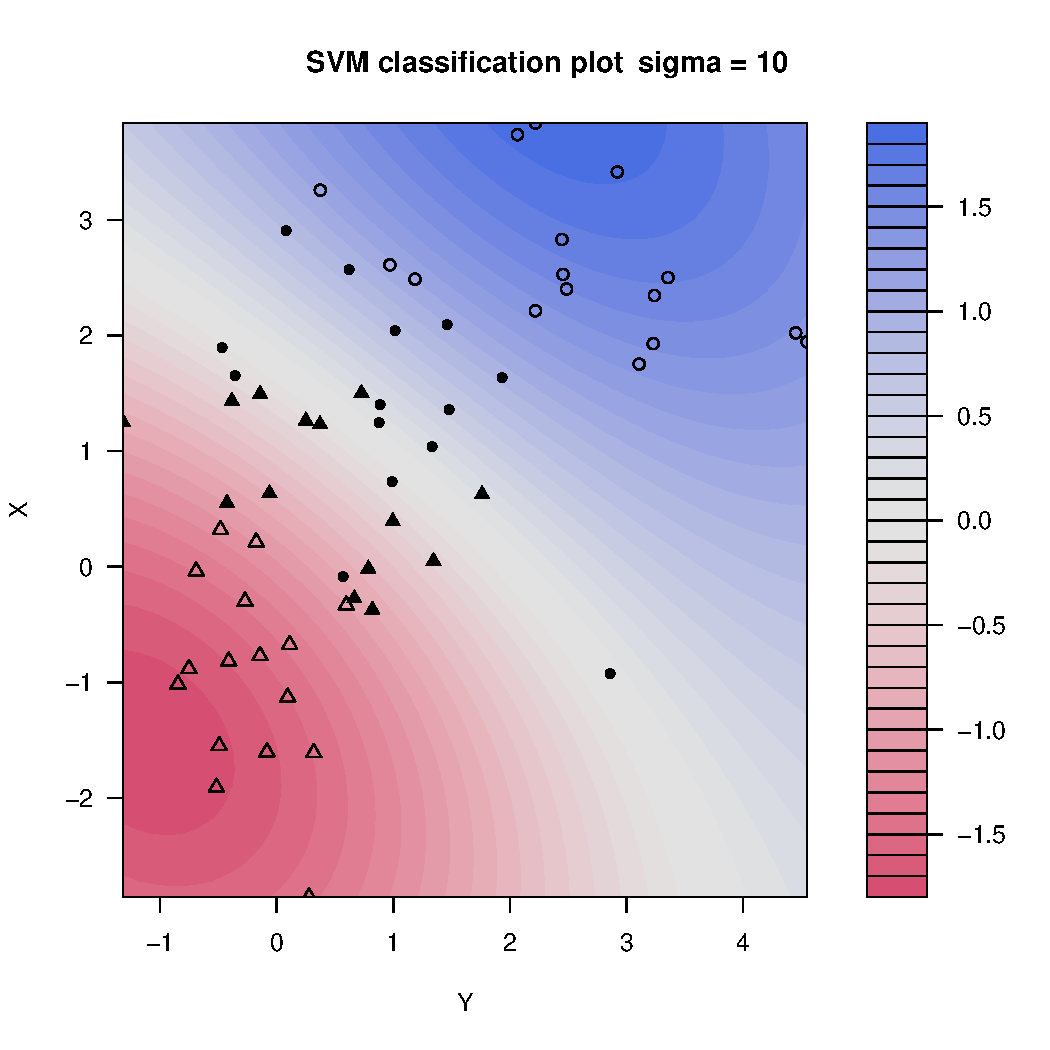
\includegraphics[width=1\linewidth]{Graphics/Problema_01/Experiment_03_3.pdf}
		\caption{$\sigma=10$}
	\end{subfigure}
	\begin{subfigure}{0.24\linewidth}
		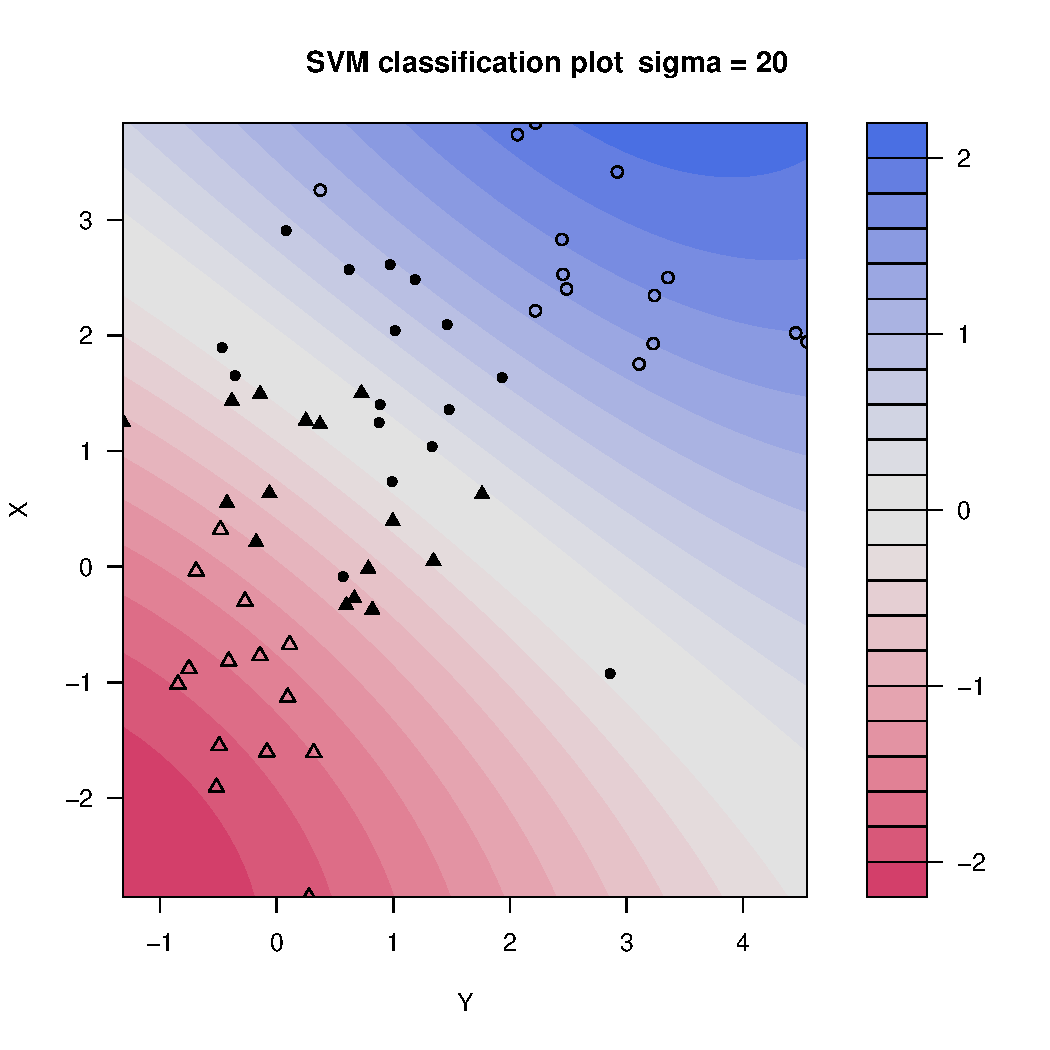
\includegraphics[width=1\linewidth]{Graphics/Problema_01/Experiment_03_4.pdf}
		\caption{$\sigma=20$}
	\end{subfigure}
	\caption{Diferentes valores para el parámetro $\sigma$ para el kernel radial.}
	\label{fig:experimento_3}
\end{figure}

En la figura \ref{fig:experimento_3} se observa que conforme se aumenta el valor de $\sigma$, el modelo de SVM con kernel radial se aproxima a tener un kernel lineal.

\subsection*{Experimento 4}

\textbf{¿Cuál es el efecto de cambiar el parámetro $\sigma$ del kernel de base radial?}

\begin{figure}[H]
	\centering
	\begin{subfigure}{0.24\linewidth}
		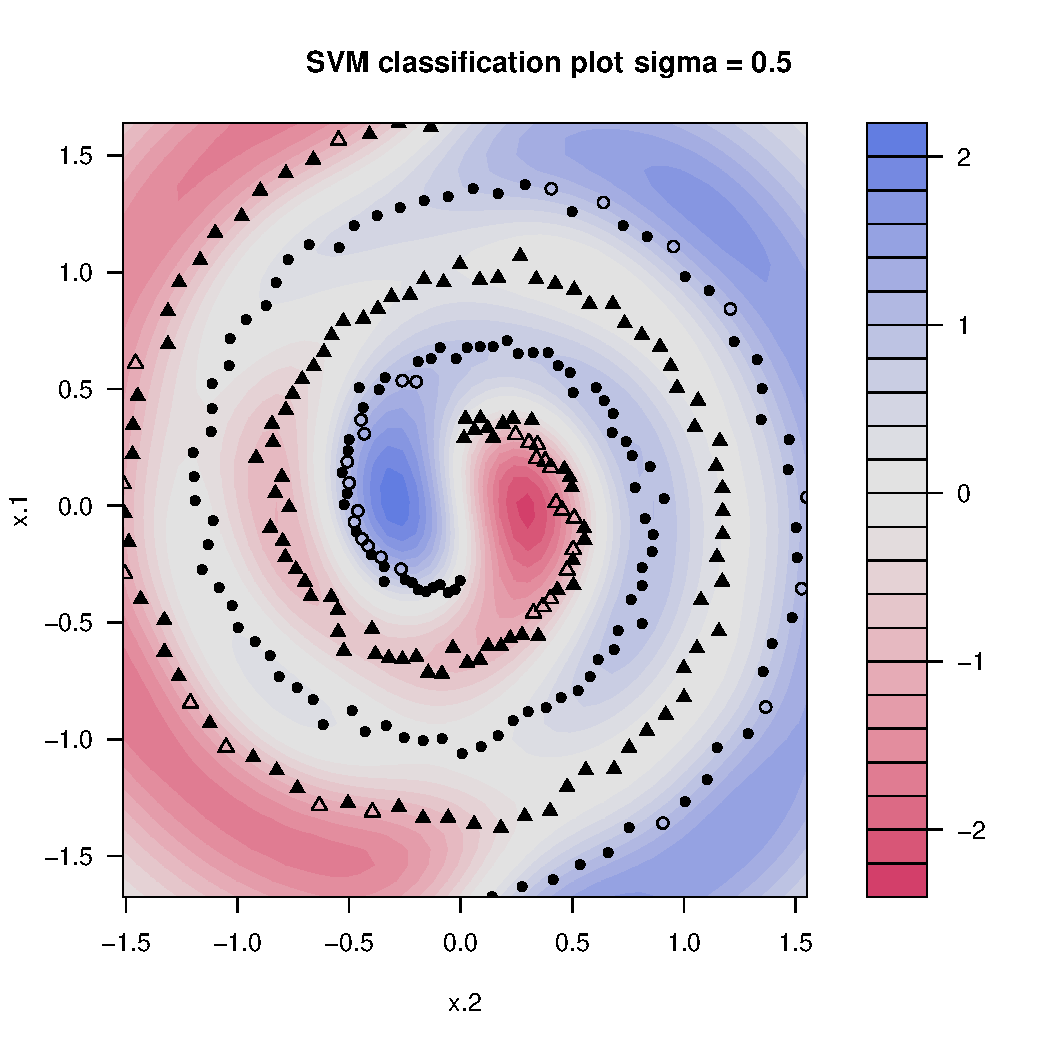
\includegraphics[width=1\linewidth]{Graphics/Problema_01/Experiment_04_1.pdf}
		\caption{$\sigma=0.5$}
	\end{subfigure}
	\begin{subfigure}{0.24\linewidth}
		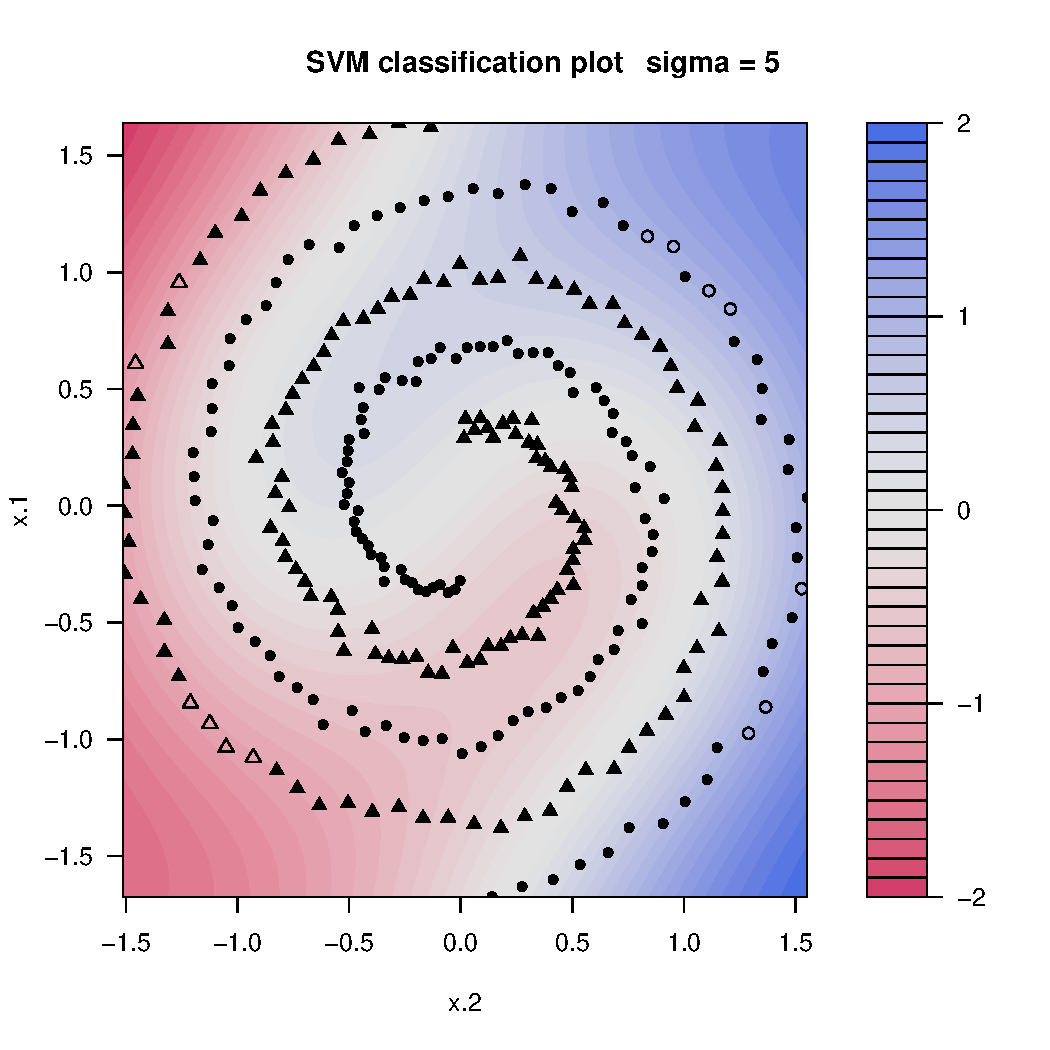
\includegraphics[width=1\linewidth]{Graphics/Problema_01/Experiment_04_2.pdf}
		\caption{$\sigma=5$}
	\end{subfigure}
	\begin{subfigure}{0.24\linewidth}
		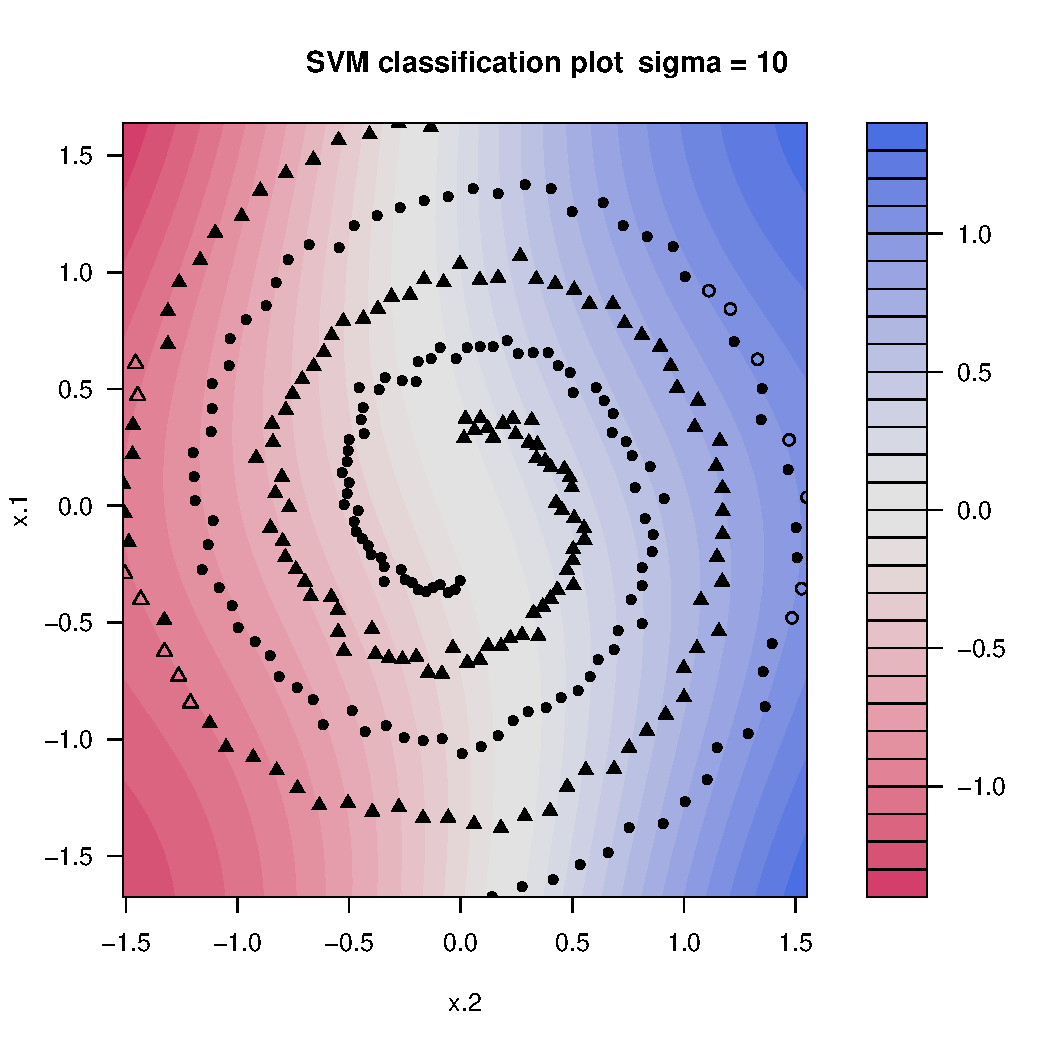
\includegraphics[width=1\linewidth]{Graphics/Problema_01/Experiment_04_3.pdf}
		\caption{$\sigma=10$}
	\end{subfigure}
	\begin{subfigure}{0.24\linewidth}
		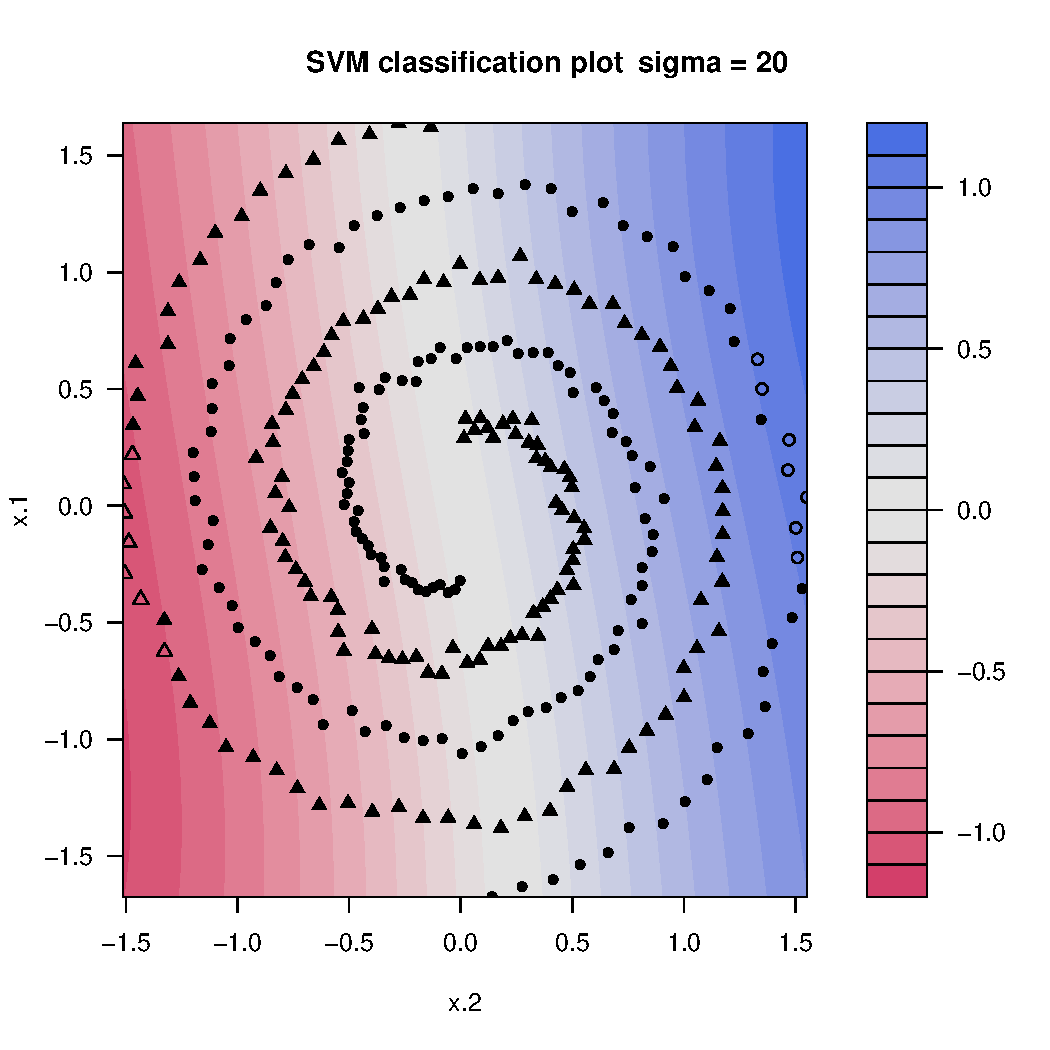
\includegraphics[width=1\linewidth]{Graphics/Problema_01/Experiment_04_4.pdf}
		\caption{$\sigma=20$}
	\end{subfigure}
	\caption{Diferentes valores para el parámetro $\sigma$ para el kernel radial.}
	\label{fig:experimento_4}
\end{figure}

En la figura \ref{fig:experimento_4} se obtienen los resultados para los diferentes valores de $\sigma$ con una base de datos dada. En esta se observa el mismo resultado que la figura \ref{fig:experimento_3}. Conforme se aumenta el valor de $\sigma$, el kernel radial se aproxima a un kernel lineal.